\documentclass[a4paper,12pt]{article} %style de document
\usepackage[utf8]{inputenc} %encodage des caractères
\usepackage[french]{babel} %paquet de langue français
\usepackage[T1]{fontenc} %encodage de la police
\usepackage[top=2cm,bottom=2cm,left=2cm,right=2cm]{geometry} %marges
\usepackage{graphicx} %'affichage des images
\usepackage{verbatim}
\usepackage{enumitem}
\usepackage{url}
\frenchbsetup{StandardLists=true}
\usepackage{hyperref}
\usepackage{perpage}
\usepackage{fancyhdr}
\pagestyle{fancy}
\renewcommand{\footrulewidth}{1pt}
\renewcommand{\headrulewidth}{0pt}
\fancyfoot[R]{\textbf Page \thepage}
\fancyfoot[C]{Simulateur d'écosystème}

\title{rapport conception}

\date{April 2022}

\begin{document}


\center
\large 
\textbf{Rapport de conception logicielle}
\vspace{1cm}
\center
Franck Willy SIMO PIUGIE\\
Celina BEDJOU\\
Ines GHOULI \\
Thierno BA \\
\vspace{1cm}
L1 Informatique\\

Groupe 1B\\

UFR-SCIENCES\\

Universite de Caen Normandie\\ 


\includegraphics[width=5cm]{images/LogoUNICAENv.png}

\center
\large 
\textbf{Simulateur d'écosystème}
\vspace{1cm}

\begin{figure}[h]
    \begin{minipage}[c]{.46\linewidth}
        \centering
        \includegraphics[width=7cm, height=5cm]{images/menu.png}
    \end{minipage}
    \hfill%
    \begin{minipage}[c]{.46\linewidth}
        \centering
        
\includegraphics[width=8cm, height=5cm]{images/logo.png}
    \end{minipage}
\end{figure}


\newpage 
\center
\renewcommand{\contentsname}{Sommaire}
\tableofcontents

\newpage
\section{Introduction}

Dans le cadre de la réalisation d'un jeu en conception logicielle, nous somme partis sur la simulation d'un écosystème. Nous avons pris ce sujet parce qu'il est complet pour la compréhension de la notion de programmation orientée objet qui, d'ailleurs est l'un des objectifs de l'unité d'enseignement. D'un autre coté, ce sujet présentait une diversité de taches à effectuer notamment la manipulation des grilles, l'outil pygame et surtout une partie expérimentale.

Pour ce projet nous devrons créer une simulation artificielle d'un écosystème mettant en exergue des êtres vivants dans une chaîne alimentaire ainsi que l'équilibre qui existe dans les milieux naturels de vie.

Notre objectif était donc dans un premier temps de créer des agents interagissant entre eux : les lions et les moutons.
Pour ces deux agents, nous devrons déterminer des propriétés spécifiques à leur espèce. Ils seront par suite mis dans un terrain à créer avec des plantes et des points d'eau.\\

Enfin, nous serons amenés à effectuer des expériences et des observations sur l'évolution du système afin de pouvoir définir des règles pour atteindre un équilibre entre les populations.


\section{Organisation du travail}
\subsection{Idées retenues}
Pour réaliser un écosystème au moyen de la programmation orientée objet tel que décrit précédemment, nous avons retenu comme idées à implémenter :
\begin{itemize}
    \item \textbf{Les Êtres en interaction}: Pour notre système nous sommes parties sur deux races d'animaux: Les lions comme prédateurs et les moutons comme proies
    \item \textbf{Les ressources alimentaires}: Il s'agit ici des points d'eau(pour que les animaux puisse s'abreuver) et des plantes pour les moutons. La ressource des lions sera les moutons traduisant ainsi l'interaction entre les deux races animales.
    \item Par la suite on aurait eu besoin d'un Terrain qui sera le support de vie de notre système.
    \item Et pour finir un monde pour contenir tout cet ensemble et pour établir les règles d'évolution du système.
\end{itemize}

\subsection{Répartition des taches}
Ce qu'il faut savoir c'est que les aptitudes des membres du groupe diffèrent d'une personne à l'autre en ce qui concerne la programmation. 
Ceci dit, pour l'organisation du travail, on se retrouvait ensemble pour élaborer des idées sur la forme à donner au projet. Ines et Thierno à la base étaient chargés de recueillir les idées adoptées pour le projet ainsi qu'à l'élaboration du diagramme de classes.
\begin{itemize}
    \item Les classes ont été élaborés par chacun des membres du groupe vu que c'était un travail assez simple; bien que d'autres attributs aient été rajoutés plutard par Celina pour la manipulation de la grille
    \item Le Terrain a été travaillé par Célina et Franck vu que les méthodes et les attributs a définir aurait été utilisés dans le monde.
    \item Les versions en console et Interface graphique du jeu ont été défini par Franck et par Celina car cette partie utilisait des algorithmes non triviaux !
    \item La version de finale de la grille a été inspirée du modèle test d'Ines
    \item La partie Expérimentale a été faite par Franck
    \item Tout au long du Travail, Ines a travaillé sur le rapport et a été rejoint par Franck vers la fin.
\end{itemize}


\section{Architecture du Projet}

\subsection{Structure du système}

Notre système étant une Biosphère en milieu terrestre, celui-ci est structuré ainsi qu'il suit :
\begin{itemize}
    \item \textbf{Le monde} définit par une classe qui représente notre système proprement dit: 
    Celui-ci est formée de populations interagissant entre elles, d'un Terrain qui est le support de vie, des ressources ainsi que des règles de vie dans le monde.
    \item \textbf{La classe Animale}: Il s'agit ici des moutons et des lions représentés par des sous-classes Herbivores et Carnivores qui hériterons de quelques attributs et méthodes de la classe Animale avec quelques spécificités telles que leur alimentation, leur mode de reproduction et leur durée de vie. Ces animaux interagiront ensemble dans une relation qui sera de prédation. L'interaction entre les animaux constitue l'un des points focal d'étude du système. En effet, toute biosphère est régie par un certains nombres d'interactions entre des êtres et dans notre cas, notre monde est plus assimilé à un système proies-prédateurs ceci parce que la gestion et l'étude du système est plus simple car on a uniquement deux populations qui interagissent.
    Les lions mangeront les moutons et cela leur fournira une valeur énergétique qui leur permettra de vivre dans le temps suivant et suivant leur sexe de se reproduire. La reproduction est conditionnée par le sexe de l'animal(féminin uniquement), l'âge et enfin son énergie interne, ainsi on est dans un cas de figure de reproduction \textbf{asexuée}.Bien que cela n'est pas en accord avec le mode de reproduction des animaux d'espèces que nous avons définis; il était question pour nous de limiter les fonctionnalités à implémenter dans notre système vu que cela allait posé un problème de temps processeur détenu par un animal. Les mêmes règles s'appliqueront au moutons mais leurs sources d'alimentations seront plutôt les plantes. Tout ces paramètres seront mieux explicitées dans la section suivante.
    \item \textbf{Les ressources}: Ce sont les plantes et les sources d'eau, leur impact ne sera pas trop immédiat sur le système car seront illimitées.
    \item \textbf{Le support de vie}: Il s'agit ici d'un Terrain représenté par une classe grille à l'intérieure de laquelle les éléments du monde seront insérés.
\end{itemize}

Ainsi la chaine alimentaire représentée peut s'écrire ainsi :

   Plantes -------> Moutons --------> Lions
  
Les plantes sont générées automatiquement, donc sont considérée comme ressource infinie.

\begin{figure}[h]
    \centering
    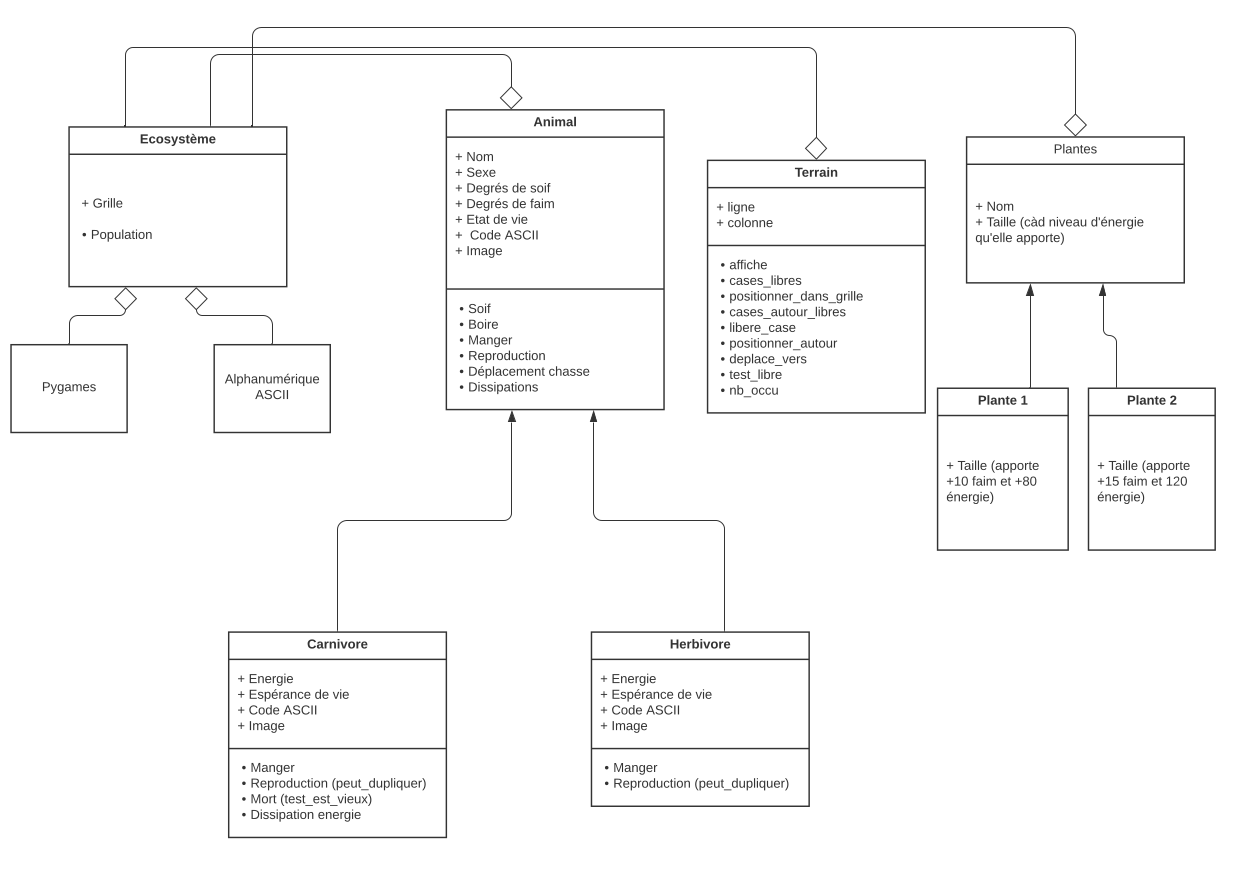
\includegraphics[width=10cm, height=5cm]{images/diagramme.png}
    \caption{diagramme de classes}
\end{figure}

\subsection{Paquetage}
Toutes les données citées précédemment ont été regroupé ainsi qu'il suit :
\begin{itemize}
    \item Un fichier Classes.py pour définir les classes Animal, Herbivore, Carnivore et Eau
    \item Un fichier grille.py pour définir la grille ainsi que toutes les méthodes qui serviront à manipuler le monde et à faciliter les interactions.
    \item Un fichier monde.py qui décrit les principales caractéristiques du monde ainsi que son contenu(ses populations, son territoire, les règles d'activités). Des spécificités seront ajoutées en fonction de la version de notre jeux.
    \item Un fichier jeu1\_0.py: qui est la première version de notre jeu faite en console avec un affichage alphanumérique des éléments du monde. La classe jeu en console sera une classe qui héritera du monde ou il y aura un polymorphisme pour la réécriture des méthodes telles que l'activité des animaux.
    \item Un fichier jeu2\_0.py: Qui est la version 2 du jeu avec affichage graphique. La classe construite héritera sera aussi une fille du monde avec une réécriture des méthodes et un rajout d'autres paramètres graphiques.
    \item A coté il y a le fichier Curve.py pour la visualisation de l'évolution des populations, le fichier menu.py pour créer un menu de notre application; le fichier config.py pour les dimensions de notre monde et pour créer les éléments qui serviront à l'interface graphique et définir l'ensemble des positions. Pour finir, nous avons d'autres fichiers et dossiers accessoires. 
\end{itemize}

\section{Construction du système}

\subsection{construction des classes}
Tous les éléments de notre système seront considérées comme des sprites.
\subsubsection{Les Plantes}
Une plante sera définie par un nom ('foin' ou 'marguerite'),sa position dans la grille (un couple d'entier), une image (carré de 10px de couleur verte pour l'interface graphique) et enfin sa taille :
\begin{itemize}
\item Taille 1 : Apporte une satisfaction de  10 au degré de faim de l'animal et +80 au niveau d'énergie.
\item Taille 2 : Apporte +15 degré de faim et +120 niveau d'énergie.
\end{itemize}

\subsubsection{Description de la classe "Animal"}
Cette classe comporte tous les éléments communs aux classes Carnivore et Herbivore, soient les fonctions et attributs suivants :\\
\begin{itemize}
    \item Attributs : Chaque animal sera défini par son nom, son degré de faim (ce sera un entier compris entre 0 et 50 qui détermine l'état de famine ou non de l'animal), son degré de soif(0-50), son sexe (1 pour féminin et 2 pour masculin) son énergie interne(entier compris entre 0 et 500).
    Il y a également x et y qui correspondent aux coordonnées de l'animal dans la grille. Une correspondance sera effectuée entre la position (x,y) dans la grille en console et (x\_,y\_) la position sur la fenêtre graphique 
    
    \item la méthode boire : A chaque fois qu'un animal boira à une source d'eau, son degré de soif sera augmenté de 20 et son niveau d'énergie sera augmenté de 45. \\
    \item La méthode soif : Si le degré de soif d'un animal est inférieur à 25, alors il aura soif. 
    \item La méthode faim : Si le degré de faim d'un animal est inférieur à 25, alors il aura faim.
    \item La méthode mort : Si le niveau d'énergie et le degré de faim sont inférieur ou égal à 0, alors l'animal meurt.
    \item Fonctions Dissipation : A chaque tour, l'énergie est diminuée de 100 (fonction "dissiper$\_$énergie"), le degré de soif est diminué de 12 (fonction "dissiper$\_$eau") et le degré de faim est diminué de 12 (fonction "dissiper$\_$aliments").
\end{itemize}

\subsubsection{Description de la classe Carnivore}
Un lion est un animal avec des propriétés spécifiques :
\begin{itemize}
    \item Initialisation : Les lions ont un niveau d'énergie écrasé à 300, quant à leurs degré de faim et de soif il sera initialisé à 25.
    
    \item Fonction Manger : A chaque mouton manger, le niveau d'énergie se verra être augmenté de 150 et le degré de faim de 25. Un lion ne pourra manger que des moutons, si celui-ci venait à essayer de manger autre chose un message "nom animal est un carnivore donc ne mange que de la viande" s'afficherait.
    
    \item Fonction Mort : Pour le maintient de l'équilibre du système, nous avons décidé que l'espérance de vie d'une lionne serait plus longue que celle d'un lion. Ainsi, un lion (sexe == 2) survivra 12 tours (c'est à dire jusqu'à 12ans) et une lionne (sexe == 1) survivra 17 tours. Pour se faire nous avons crée la fonction "test$\_$est$\_$vieux" qui s'ajoutera à la condition définie par la fonction mort de la classe Animal.
    
    \item Fonction Reproduction : Aussi appelée "peut$\_$dupliquer", cette fonction est essentielle à l'évolution notre système. Un lion peut se reproduire à condition que ce soit une femelle (sexe == 1), que son niveau d'énergie soit supérieur ou égal à 315 et que son âge soit supérieur ou égal à 5ans. 
    
\end{itemize}

\subsubsection{Classe Herbivores}
Un mouton est un animal avec les spécificités suivantes :
\begin{itemize}
    \item Initialisation : généralement, les moutons auront au début un niveau d'énergie de 250, un degré de faim et de soif de 20.
    
    \item Fonction Manger : Un mouton ne peut se nourrir que de plantes. Selon le niveau de la plante (cf Objet Plante) il gagnera soit +80 en énergie et 10 en degré de faim, soit 120 en énergie et 15 en degré de faim.
    
    \item Fonction Reproduction : De la même manière que pour les carnivores, un mouton peut se reproduire si c'est une femelle et si il a au moins 5 ans, à la seule différence que le niveau d'énergie doit être supérieur ou égal 320.   
\end{itemize}

Nous avons aussi les points d'eau essentiellement caractérisée par leur position dans la grille

\subsection{Le Terrain}
    La construction se fait à l'aide des dimension (un nombre de lignes et un nombre de colonnes),puis on initialise une grille de dimension ligne x colonne avec du vide (\_) représentant la terre. Les méthodes essentielles de la grille sont :
    \begin{itemize}
        \item Positionner dans grille: qui prend un élément ayant un attribut position (x,y) et le fixe dans la grille à la position (x,y)
        \item Cases libres : Qui retourne la liste de couples de cordonnées correspondant aux positions libre du terrain
        \item Cases autour libres : C'est une méthode qui prend en paramètre un élément du système et retourne les positions autour de l'animal qui sont libres
        \item Libère\_case : Prenant en paramètre un élément du du terrain et libère de sa position
        \item L'affichage de la grille pour la version alphanumérique: Des caractères sont utilisés pour afficher chaque élément de l'écosystème.
    \end{itemize}


\subsection{Le monde}
Les attributs de la classe monde sont :
\begin{itemize}
    \item Deux listes pour contenir la population des animaux: une pour les moutons et une autre pour les animaux. La liste est choisie par rapport au dictionnaire parce que la liste sera constamment modifiée par la naissance de nouveau animaux et la mort d'autres.
    \item Une liste pour les plantes, une autre pour les points d'eau.
    \item Un terrain qui est construit à partir du constructeur de Terrain défini dans grille.py.
    \item d'autres petits attributs pour faciliter la gestion du monde
\end{itemize}

Les méthodes :
\begin{itemize}
    \item L'initialisation des lion: qui consiste à ajouter 3 lions à la liste des lions
    \item L'activité des moutons qui est un ensemble d'opérations: Si l'animal a soif, il faut choisir aléatoirement un point d'eau et le positionner autour et exécuter la fonction boire de l'animal, quant il aura faim il faudra choisir une plante et le déplacer à la position de la plante et exécuter sa fonction manger. Par la suite, on teste si l'animal rempli les conditions pour se reproduire(défini plus haut), si oui, on choisi une position aléatoire qui est libre autour de l'animal et on crée un nouvel être qu'on le positionne dans le terrain et qu'on rajoute dans la liste des moutons et enfin le niveau d'énergie de l'animal parent se décrément de 120 (énergie dissipée pour la reproduction). Après ceci, on incrémente l'âge de l'animal et on exécute la fonction de dissipations et puis on test si l'animal est mort ou pas.
    \item L'activité des lions : similaire à celle des moutons à la différence que le lion lui choisira un mouton aléatoirement parmi la liste des moutons en vie.
    \item La régénération des plantes : Qui consiste à générer aléatoirement un nombre de plantes dans la grille en fonction des versions du jeu. cette méthode sera exécutée lorsque le nombre de plantes sera réduit.
    \item La régulation de la population des lions : Malgré le fait que les lions ont été assignés une espérance de vie, leur accroissement était assez rapide et la conséquence était l'extinction des moutons et par conséquent la leur aussi. subséquemment, nous avons décider de faire un test pour vérifier à chaque fois que la population des lions s'approche de trop près de celle des moutons, et par la suite nous abattons un nombre de lions.
\end{itemize}

Après définition des attributs et méthodes qui permettront l'évolution du monde, le fonctionnement du monde est ainsi: On initialise 2 moutons de sexe féminin. On les mets en activité et elles se reproduisent assez rapidement jusqu'à atteindre le nombre de 20 moutons, à cet instant, nous exécutons le code d'initialisation des lions (3 lions) puis on laisse le système évoluer et à chaque cycle, on effectue des test pour voir s'il faut une régénération des plantes et aussi s'il faut réguler le système.

\subsection{Les deux version du jeu}
\subsubsection{Alphanumérique}
Cette version est assez basique, elle est le résultat de l'application directe des règles citées plus haut et de l'affichage alphanumérique après chaque tour d'activité des animaux ainsi que statistiques de système.
\begin{figure}[h]
    \centering
    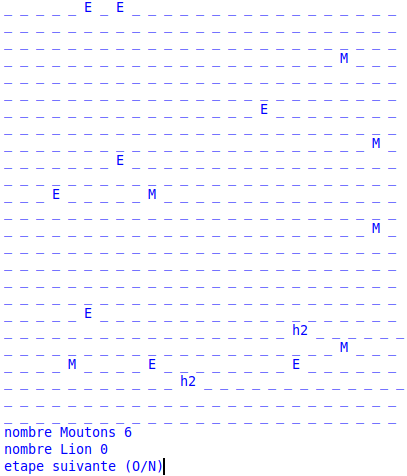
\includegraphics[width=7cm, height=4cm]{images/console.png}
    \caption{Affichage en console}
\end{figure}
\subsubsection{La version avec Interface graphique}
Elle se base sur la version Alphanumérique qui est est exécutée en background pour effectuer les algorithmes et les test mais effectue plutôt un affichage graphique avec implémentation du déplacement des animaux. D'autres outils de décoration viennent s'ajouter à cette version. On utilise le fichier config pour répartir la fenêtre graphique.
Une section est reservée à la simulation de l'écosystème où les positions du terrain sont dans le fichier config.py qui est un dictionnaire ayant pour clé les positions dans la grille et pour valeur la position sur la fenêtre graphique. Et grâce à ces données, une animation graphique est effectuée avec pygame.

À coté de la version graphique, nous avons menu pour notre logiciel.

Pour lancer le jeu, il faudra exécuter le menu.

\begin{figure}[h]
    \begin{minipage}[c]{.46\linewidth}
        \centering
        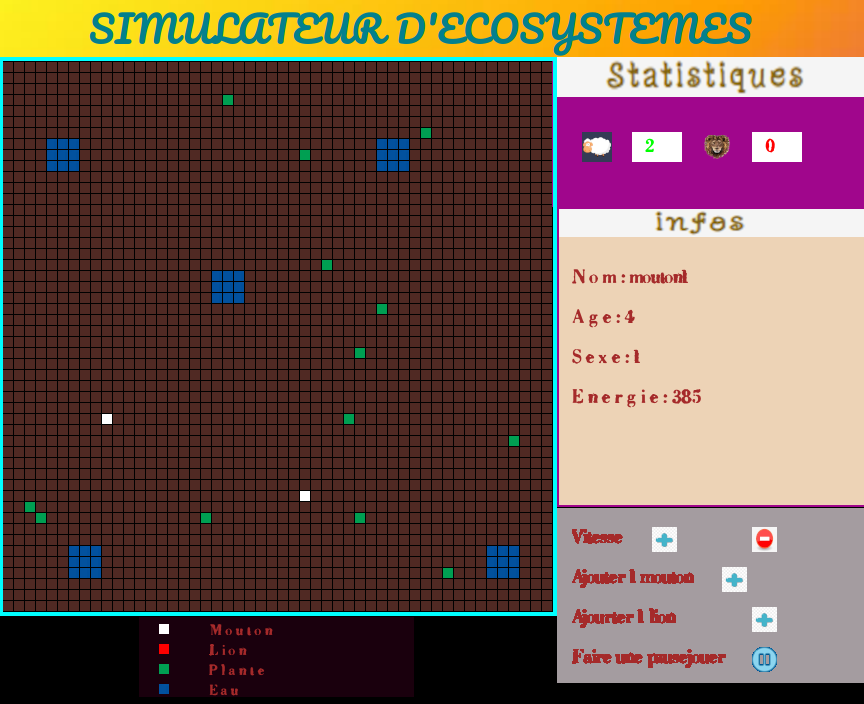
\includegraphics[width=8cm, height=5cm]{images/interface.png}
        \caption{La fenetre de la la simulation de l'écosysteme}
    \end{minipage}
    \hfill%
    \begin{minipage}[c]{.46\linewidth}
        \centering
        \includegraphics[width=8cm, height=5cm]{images/menu.png}
        \caption{Le Menu}
    \end{minipage}
\end{figure}
La courbe sur le menu permet d'effectuer une animation matplotlib des courbes de variations des deux populations.

\subsection{Algorithmes utilisés}
L'un des points essentiel de la version graphique est l'algorithme de déplacement pour les différents animaux. Pour notre système, nous avons utilisé deux principaux algorithmes presque similaires pour le déplacement.

\subsubsection{le déplacement}
Pour déplacer un animal de la position (x,y) à la position (a,b), on effectue une incrémentation ou une décrémentation successive de x et ou de y suivant que (x > a ou x < a) et (y > b ou y x < b) jusqu'à ce qu'on arrive à (x=a et y=b).
à chaque pas d'incrémentation ou de décrémentation, on affiche l'animal à sa nouvelle position tout en libérant l'ancienne.
Par exemple, pour quitter de la position (2,3)  à la position (0,7) on passe par les positions suivantes (2 - 1,3 + 1)=(1,4) ------> (1-1,4+1)=(0,5) ------> (0,5+1)=(0,6) ------> (0,6+1)=(0,7).

Toutefois, les déplacement ne sont pas aussi simples, il peut arriver qu'une case sur le chemin soit occupée, ainsi donc on distingue deux types de déplacement :

\begin{itemize}
    \item \textbf{Déplacer un animal pour qu'il puisse s'abreuver: } Pour s'abreuver l'algorithme choisi une position (a,b) libre autour d'une source d'eau qui sera la destination.
Et on fait l'animal contourner les obstacles de toute nature (animal,plante..;.) sur le chemin.

Ce qu'il faut savoir c'est qu'à chaque position d'un animal, il y a 8 cases autour de lui

\begin{figure}[h]
    \centering
    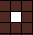
\includegraphics[width=4cm, height=3cm]{images/cases.png}
    \caption{positions autour d'une position}
\end{figure}

Une de ces cases est sur son chemin. Si cette case est occupée, l'animal choisira autre une position autour de lui(qui est libre) tout en restant dans l'algorithme pour la destination (a,b).
Ainsi nous faisons l'animal éviter tous les obstacles sur son chemin jusqu'à destination d'un point pour s'abreuver.

Ainsi pour reprendre l'exemple de déplacement précédent, on suppose maintenant qu'il y a un obstacle à la position (0,5), une route emprunté par l'animal est :
(2,3) -------> (1,4) -------> (0,4) ------>(0+1,4+1)=(1,5) ------> (0,6) -------> (0,7)
On peut voir que lorsque l'animal est arrivé à (0,4), il ne pouvait pas aller en (0,5) et a plutôt pris une position autour de (0,4) soit (1,5) par exemple.
\textbf{NB}: le chemin dans ce cas de figure n'est plus unique.

Et pour éviter que l'animal perde trop de temps sur un obstacle, nous avons défini une liste piste\_déjà contenant toute les positions occupées par un animal au cours de son déplacement et on s'est rassurer qu'il n'occupe pas une même case plus de 10 fois.

    \item \textbf{Déplacer un animal pour qu'il puisse manger: } Pour manger, un animal a besoin d'une ressource selon son régime alimentaire ainsi que de la position (a,b) de la ressource qui sera éventuellement sa destination finale.
    Le même principe du déplacement pour boire est presque appliqué au déplacement pour manger à la différence que l'animal va esquiver sur son chemin tout ce qui n'est pas la ressource nécessaire pour lui. Toutefois, il peut arriver qu'en cours de route, il trouve sur son chemin une ressource de nature qu'il recherche, quand c'est le cas, la destination finale de l'animal est modifiée et remplacée par la celle de la ressource proche de lui et ainsi on sort plus tôt  de l'algorithme.
\end{itemize}


\section{Les compléments de l'interface}
\subsection{Informations sur l'évolution du système}
Pour une bonne compréhension du jeu, nous avons ajouté un cadre réserve aux statistiques de la simulation qui affiche le nombre de moutons et celui des lions.

Juste en dessous, il y a une section  "infos" réservée à afficher les caractéristiques internes des éléments du monde lorsqu'on clique sur un.
Pour un Animal par exemple, après un clic, on affichera son nom (il s'agit de son espèce (mouton ou lion)suivit d'un numéro indiquant le quantième animal il est de sa race),ensuite sont âge, son sexe (1 ou 2) et enfin son énergie interne.

En dessous du monde et de son évolution, il y a une légende explicative des différents carré sur la simulation.

\subsection{Interaction avec l'utilisateur et perturbation}
\begin{itemize}
    \item Nous avons rajouté deux boutons (+) et (-) pour accélérer respectivement ralentir la vitesse du jeu.
    \item Pour la perturbation, nous avons rajouté deux boutons pour ajouté un mouton ou lion dans le système.
\end{itemize}


\section{Expérimentations et équilibre}
Dans le but de mieux comprendre l'évolution de notre système, nous avons effectué des expériences pour déterminer certains paramètres qui nous auront servi à vérifier si notre écosystème respectait l'équilibre des systèmes proies-prédateurs traditionnels. Pour ce faire, nous sommes partis sur le modèle proies-prédateurs de LotKa-Voltera qui décrit un couple d'équations permettant de décrire la dynamique d'un système proies-prédateurs. Les équations s'écrivent ainsi qu'il suit :
\begin{equation}
    \lbrace_{\frac{dy(t)}{dt}  =  y(t)(cx(t) - d)} ^{\frac{dx(t)}{dt} = x(t)(a - by(t))}
\end{equation}
Ou x(t) est l'effectif des proies, y(t) celui des prédateurs les coefficients a,b,c et d à déterminer expérimentalement :
\begin{itemize}
    \item a le coefficient d'accroissement des proies indépendemment de prédateurs:
    \item b le taux de mortalité des proies du aux prédateurs
    \item c le coefficient d'accroissement des prédateurs en fonction des proies disponibles
    \item d le coefficient de mort des prédateurs en l'absence des proies
\end{itemize}

\subsection{Détermination du coefficient a}
Pour déterminer le coefficient a, nous avons créer un monde avec deux moutons(proies de notre système) que nous avons laisser évoluer sur une longue période et avons observer la courbe d'évolution en fonction du nombre d'activité et par la suite nous avons fait un ajustement linéaire de la courbe et puis calculer la pente de la droite de régression.

\begin{figure}[h]
    \begin{minipage}[c]{.46\linewidth}
        \centering
        \includegraphics[width=8cm, height=5cm]{images/code1.png}
        \caption{code}
    \end{minipage}
    \hfill%
    \begin{minipage}[c]{.46\linewidth}
        \centering
        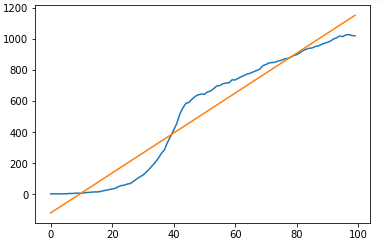
\includegraphics[width=8cm, height=5cm]{images/courbe1.png}
        \caption{Aspect de la courbe 1}
    \end{minipage}
\end{figure}

Cette Opération a été effectuée 10 fois et les pentes ont été enregistrés dans la liste scores; les coefficient variaient entre 11 et 12;

\subsection{Détermination du coefficient b}
Nous avons créer un nouveau monde avec 20 moutons et 3 lions et par la suite nous avons mis uniquement les lions en activité et avons observée la courbe de décroissance du nombre de moutons et par la suite avons effectué un ajustement linéaire la courbe et avons récupérer la valeur absolue de la pende de la droite de régression linéaire.
(On n'affichera pas tous les codes)
\begin{figure}[h]
    \centering
    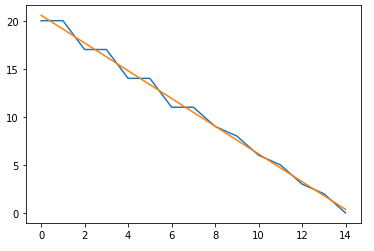
\includegraphics[width=10cm, height=5cm]{images/courbe2_.png}
    \caption{courbe 2}
\end{figure}

\subsection{Détermination des coefficients c et d}
Pour déterminer c, nous avons créer un monde normal(tout en se rassurant de la présence suffisante de proies) et dès l'apparition des prédateurs nous avons récupérer la courbe de leur évolution. Cette opération a été effectuée 10 fois afin de récupérer la courbe qui présente une croissance normale et avons déterminée la pente.
Pour le coefficient d, on a créer un autre monde avec 100 prédateurs(lions) sans aucun mouton et avons laissé le système évoluée et observé la décroissance de la population des prédateurs:

\begin{figure}[h]
    \begin{minipage}[c]{.46\linewidth}
        \centering
        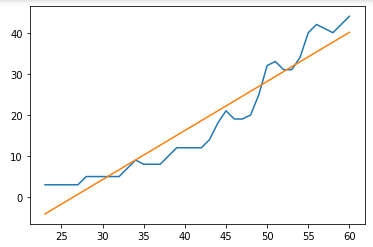
\includegraphics[width=8cm, height=5cm]{images/courbe3.png}
        \caption{Détermination de c}
    \end{minipage}
    \hfill%
    \begin{minipage}[c]{.46\linewidth}
        \centering
        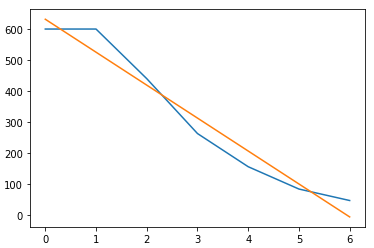
\includegraphics[width=8cm, height=5cm]{images/courbe2.png}
        \caption{Détermination de d}
    \end{minipage}
\end{figure}

\subsection{Résultats}
Après avoir effectué ces opérations, les coefficients obtenus en valeur absolues sont ainsi qu'ils suivent:

\begin{itemize}
    \item a = 12.571290729072915
    \item b = 1.4428571428571428
    \item c = 1.3156800525221573
    \item d = 17.785714285714285
\end{itemize}

La condition d'équilibre dans ce système est qu'a chaque instant 

\begin{equation}
    \lbrace_{\frac{dx(t)}{dt} = 0}^{\frac{dy(t)}{dt} = 0}
\end{equation}

 Chose que notre système ne respectait pas d'ailleurs; ce qui traduit une imprécision dans le calcul des coefficients a,b,c et d et aussi le fait que notre système tel que définit ne pouvait pas s'équilibrer.

\begin{figure}[h]
    \centering
    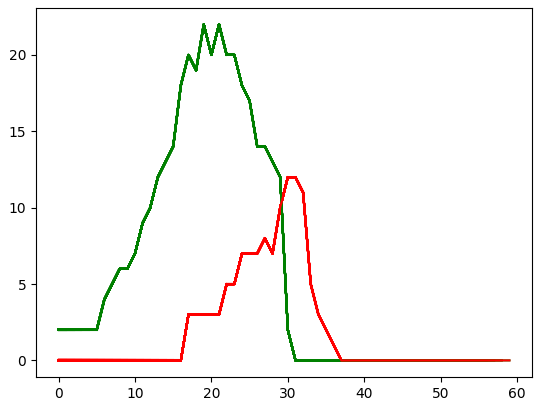
\includegraphics[width=10cm, height=5cm]{images/non_eq.png}
    \caption{Évolutions des deux populations du système sans régulateur}
\end{figure}

On observe clairement que la population des proies augmente jusqu'à un seuil (24) pour le cas de figure et par la suite la population des prédateurs augmente également et par conséquent le nombre de proies dévorées aussi. La situation se termine par une extinction proies suivie de celle des prédateurs(par manque de de proies à manger).

\subsection{Résolution}
Pour éviter l'extinction d'une quelconque population et au regard des expériences menées, nous avons rajouter de nouvelles règles pour la reproduction au sein de chaque population. Ajouté à cela , nous avons doter notre monde d'une méthode régulatrice pour s'assurer que la population des prédateurs ne venait jamais à dépasser celle des proies.

\begin{figure}[h]
    \begin{minipage}[c]{.46\linewidth}
        \centering
        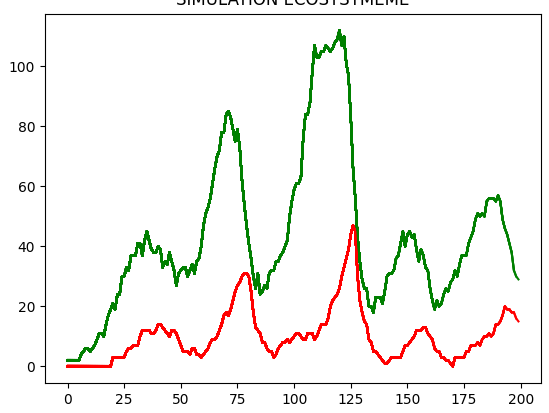
\includegraphics[width=8cm, height=5cm]{images/eq.png}
        \caption{Évolution des populations avec régulateur}
    \end{minipage}
    \hfill%
    \begin{minipage}[c]{.46\linewidth}
        \centering
        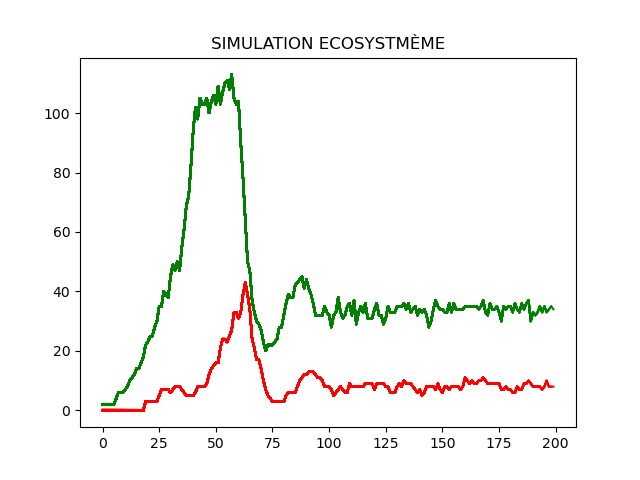
\includegraphics[width=8cm, height=5cm]{images/particu.png}
        \caption{Phénomène particulier}
    \end{minipage}
\end{figure}

Sur la figure 7, on s'est permis de faire une simulations sur 200 tours(200années) et il y a eu aucune extinction de population.
Cependant, la figure 8 présente un phénomène assez particulier: à partir de l'année 100 , les courbes des populations varient très peu; il y a une sorte de stabilité. Ceci veut tout simplement dire qu'à partir de l'année 100 le système s'équilibre tout seul sans utiliser de régulation.

Au sorti des expériences menées, nous pouvons conclure que notre système s'équilibre lorsque la différence entre le nombre de moutons et de lion est d'environ de 27 et que le nombre de lions varie entre 7 et 11.

\section{Conclusion}
Dans le but de réaliser une simulation artificielle d'un écosystème, tout au long de notre projet, nous avons créer des objets "Animal", "Carnivore" , "Herbivore" et "Plante" et par la suite nous avons créer un objet "Monde" qui possède un Terrain (grille) comme support de vie à l'intérieur duquel les animaux menaient leur activité de vie. Nous avons fini par trouver une condition d'équilibre à notre système.

Toutefois, le monde que nous avons créer est un monde ordonné où le processeur est attribué à chaque être afin qu'il puisse réaliser son activité avant de le passer à un l'être suivant. Ce qui rend le temps de simulation pas terrible. On aurait aimer améliorer le jeu afin que chaque être puisse se déplacer simultanément tout en exécutant les algorithmes implémentés avec leur mise à jour.

\newpage
\appendix
\section{Sources}

\begin{itemize}
    \item Pour réaliser ce projet, nous nous sommes inspirées des exemples faits en cours et aussi pour les la gestion de la fenetre graphique avons regardé quelques tutos youtube notemment pour la simualtion avec matplotlib et la création du Menu.
    \item Pour la phase expérimentale, nous sommes inspirés des équtations de de Lotka-Voltera tiré sur  \href{https://fr.wikipedia.org/wiki/\%C3\%89quations_de_pr\%C3\%A9dation_de_Lotka-Volterra}{Wikipédia}
\end{itemize}

\end{document}
